\chapter{Mixer Page:}
The mixer page graphically illustrates the Volume Levels of the sixteen MD tracks of the current Kit.\\
\\
The trigger interface is used in conjunction with encoders to raise or lower the volume of multiple tracks simultaneously.\\
\\
\fbox{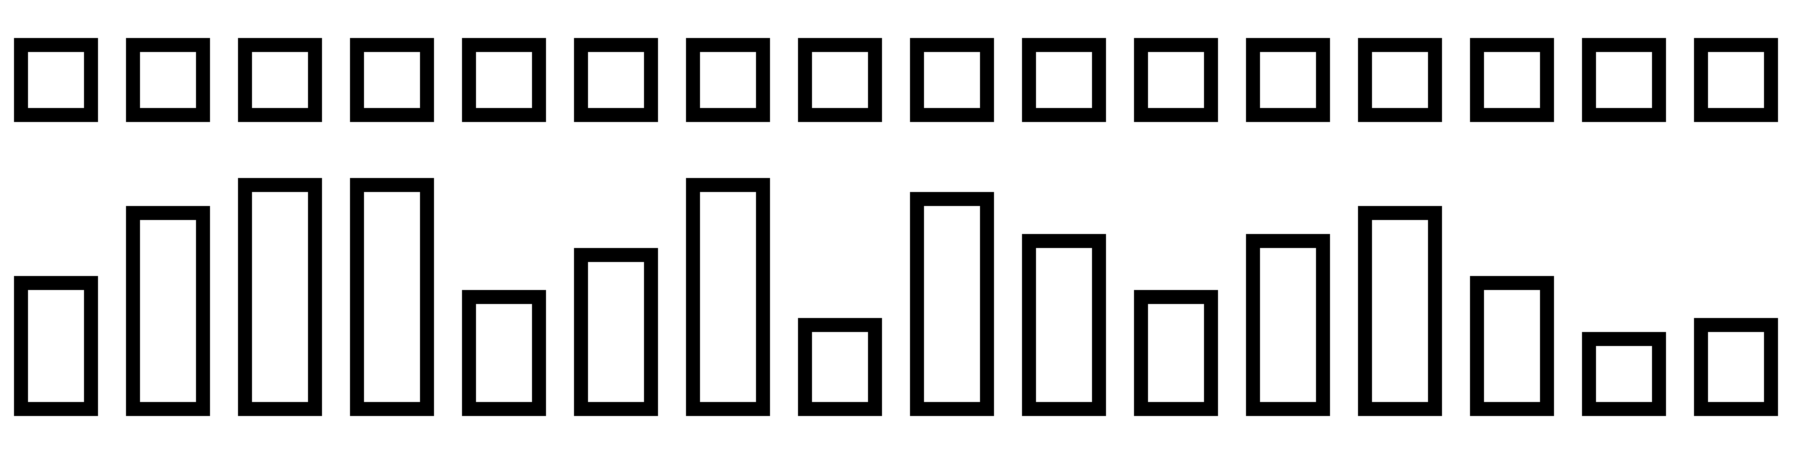
\includegraphics[scale=.40]{mixer_page_init.png}}\\\\
\textit{The Mixer Page is accessible from the PageSelect page.Pressing \textbf{[ Save] } from within the Mixer Page  allows you to toggle between the Mute and Mixer pages.}
\subsection{Encoder Assignment:}
\begin{itemize}
	\item \textbf{[ Encoder 1 ]: } Level
	\item \textbf{[ Encoder 2 ]: } Level
    \item \textbf{[ Encoder 3 ]: } Level
	\item \textbf{[ Encoder 4 ]: } Level
\end{itemize}


\subsection{Toggling Mutes}
The top row of mixer page shows the mute state of each Track. \\
\\
Holding down \textbf{[ Write ]} and pressing a trigger button on the MD allows you to quickly toggle the mute state of a track\\
\\
\textit{Note: There is no method of detecting Mute changes that occur from the MD's mute window, MCL attempts to learn the mute state as  MIDI notes are detected.}
